\chapter{The ATLAS Trigger System}
\label{ch:trigger}
\epigraph{\emph{Software is a great combination between artistry and engineering.}}{Bill Gates}
%\epigraph{\emph{Engineering. Where the noble semiskilled labourers execute the vision of those who think and dream. Hello, Oompa-loompas of science.}}{Sheldon Cooper}

	The \ac{ATLAS} trigger system together with its performance will be presented in this chapter. A brief introduction about the reason behind the need of a trigger system, together with its implementation in \ac{ATLAS}, will be discussed in Section~\ref{sec:Trig_intro}. The \ac{L1} trigger and \ac{HLT} will be discussed in Sections~\ref{sec:L1} and~\ref{sec:HLT}, respectively. Finally, Section~\ref{sec:Trig_perf} will be dedicated to the performance of \ac{HLT} for low-\pt\ single-lepton, and medium- and high-\pt\ \bj\ triggers - which has been part of the \textit{qualification task}\footnote{In order to become an \ac{ATLAS} author, a person must have been an active \ac{ATLAS} member for at least one year working on a technical work} of the author -, together with the performance of the missing transverse energy trigger, \met, - as the most relevant trigger for the analysis discussed in Chapter~\ref{ch:stop_ana}.



	\section{Overview}
	\label{sec:Trig_intro}

		More than 80 \ifb\ of \pp\ collisions were delivered in 2016 and 2017 by the \ac{LHC} and, due to storage space limitations, it is not feasible to save all the information about the collision after every bunch crossing, so the \ac{ATLAS} Trigger System is indispensable to reduce the read-out rate to a sensible value without affecting the physics programme of \ac{ATLAS}, \eg\ discarding potentially interesting events. A multiple-level architecture is employed to allow the trigger enough time to identify interesting events, using both software- and hardware-based real-time algorithms. 

		Figure~\ref{fig:TDAQSyst} shows the \ac{TDAQ} system. This is comprised of both a hardware-based first-level trigger (\ac{L1}) and a software-based \ac{HLT}, as already mentioned in Section~\ref{sec:trigSyst}. The \ac{L1} trigger decision is formed by the \ac{CTP}, which receives inputs from the \ac{L1Calo} and \ac{L1Muon} triggers. Once the events pass the \ac{L1} selection, they are buffered in the \ac{ROS} and processed by the \ac{HLT}, which receives information on the \ac{RoI} from \ac{L1} to be used for track reconstruction in the trigger algorithms.
		%\footnote{A Region of Interest is an $\eta-\phi$ region within the \ac{ATLAS} detector identified by the \ac{L1} Trigger}
		An \ac{RoI} is an extended wedge-shaped spatial region in the detector, consisting of a direction in $\eta-\phi$ originating from a $z$-position along the beam-line, extended along the beam-line by independent directions with respect to this $z$ position, and extended about the $\phi$ direction with independent directions in pseudo-rapidity, at the maximum and minimum $z$ positions along the beam-line. %In other words, an RoI is not just a simple inverted pyramid with the apex on the beam-line, but a wedge extended along the beam-line, since the $z$ vertex position is not known until after the tracking has taken place, so the \ac{RoI} must be extended along the full length of the interaction region at the beam-line.	%%% ROI DEFINITION Events accepted by \ac{HLT} are then transferred to local storage and exported to the \emph{Tier-0} facility at CERN’s computing centre for offline reconstruction.

		\begin{figure}[!htb]
			\centering
			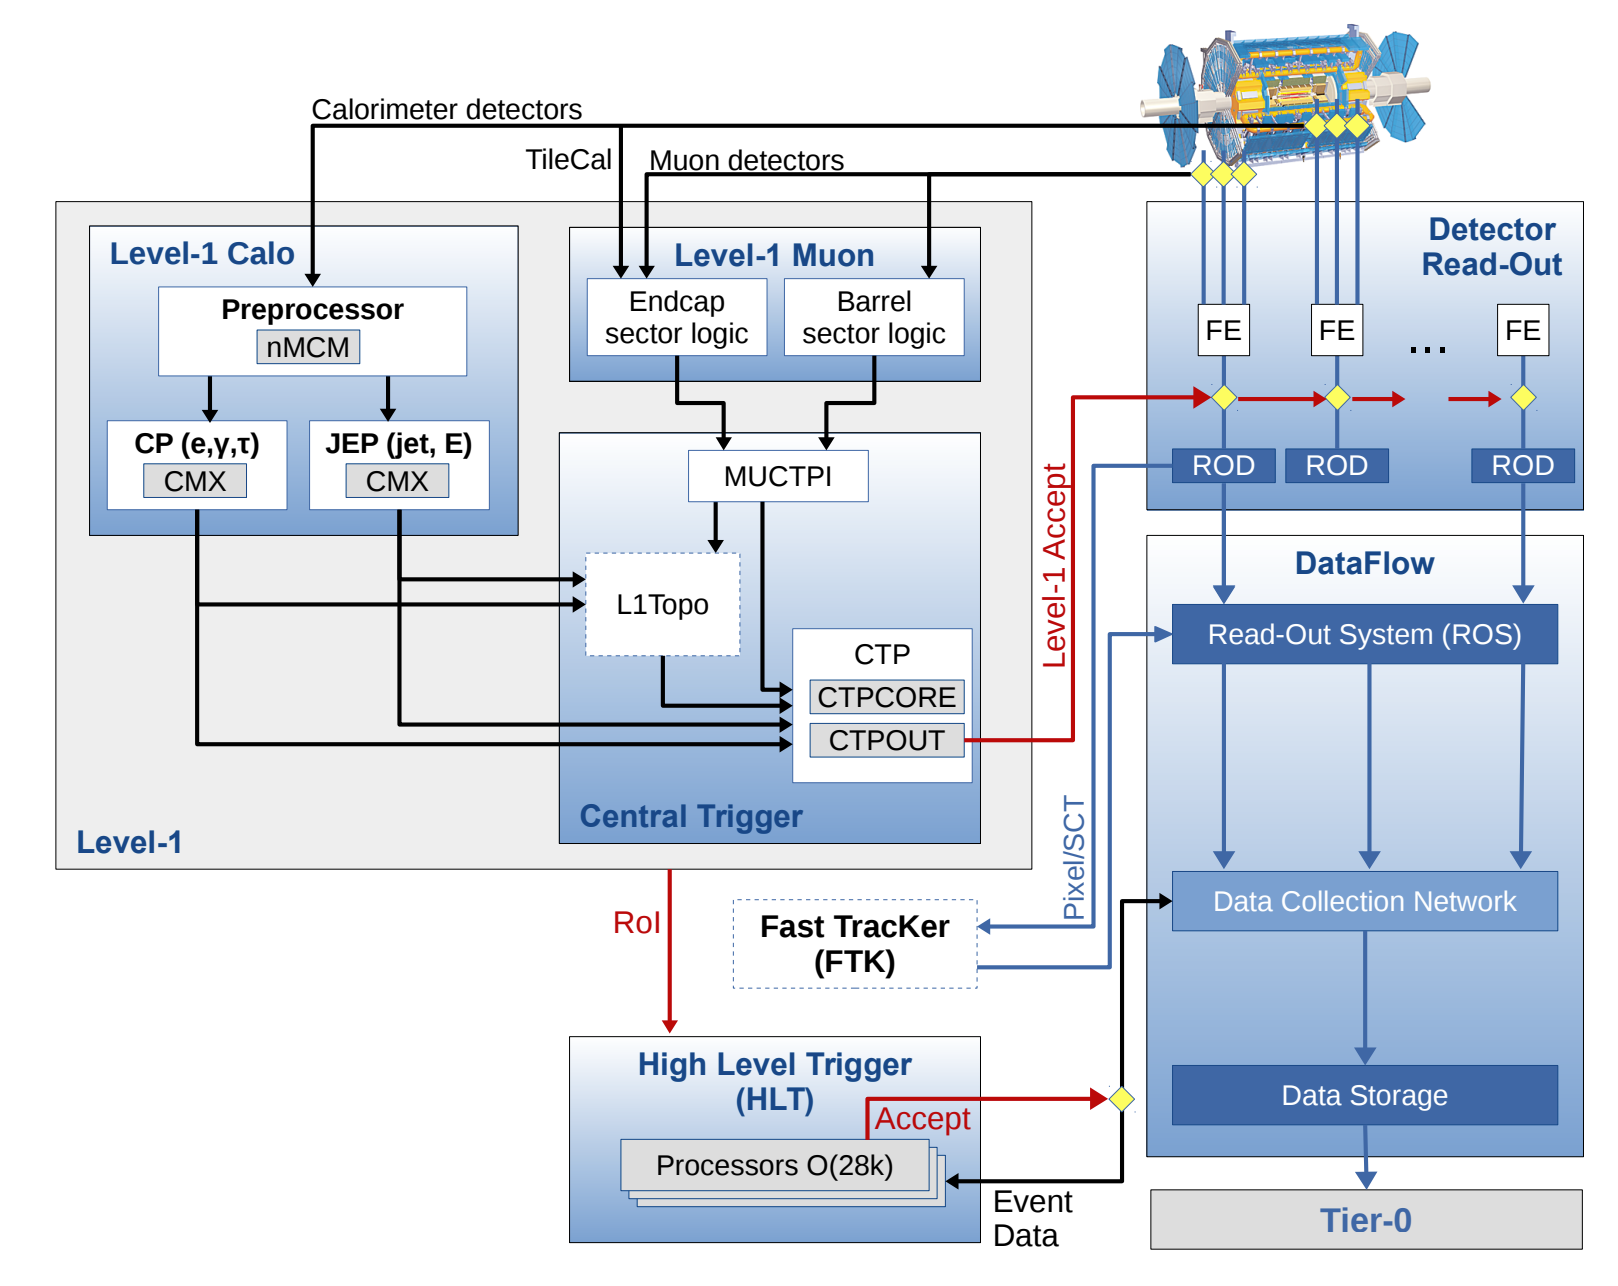
\includegraphics[width=\textwidth]{Detector/Trigger/TDAQSystem}
			\caption{The \ac{ATLAS} \ac{TDAQ} system. \acs{L1Topo} and \ac{FTK}~\cite{ATLASTrigger2015} have not been used for the results shown in this thesis.}
			\label{fig:TDAQSyst}
		\end{figure}

		The trigger system is configured via the so-called trigger \textit{menu} which contains the multiplicity requirement (number of tracks) and the pre-scale factors\footnote{A factor associated with a trigger at each level that indicates what fraction of events, that could pass this trigger selection, is actually accepted.}. Additionally, the menu is meant to define the trigger \textit{chains} - usually referred to just as trigger - that start from a \ac{L1} trigger and specify a sequence of reconstruction and selection steps for the specific trigger signatures required in the trigger chain. This is named after the following convention: 

		$$\mathrm{TriggerLevel\_TypeAndThreshold\_Identification\_Isolation}$$

		\noindent Here, ``TriggerLevel'' refers to either \ac{L1} or \ac{HLT}, ``TypeAndThreshold'' refers to the type of object to trigger on (electron, muon, \met, etc.) and its energy threshold. If any identification and/or isolation criteria are included, these are appended at the end of the name: \texttt{HLT\_e24\_lhmedium} is an electron trigger with a $24$ \GeV\ threshold, using ``medium'' identification criteria, which will be further discussed in Chapter~\ref{ch:evSimObjReco}. 
		% Figure~\ref{fig:trig_chain} shows an illustration of an electron-trigger chain used to select electrons \cite{ATLASTrigger2010}.

		% \begin{figure}
		% %\begin{wrapfigure}{L}{.5\textwidth}
		% 	\centering
		% 	%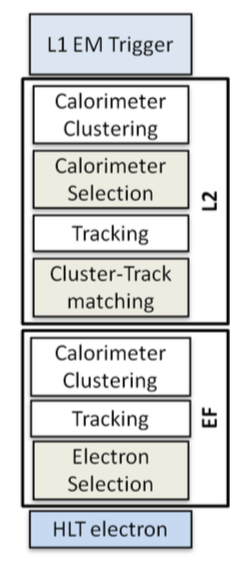
\includegraphics[height=.3\textheight]{Trigger/trig_chain}
		% 	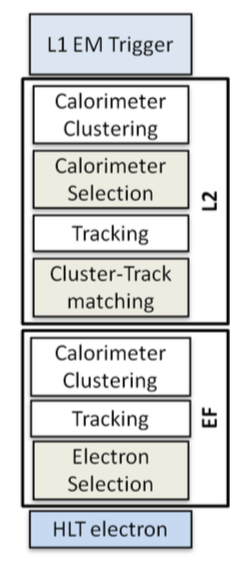
\includegraphics[width=.3\textwidth]{Trigger/trig_chain}
		% 	\caption{\label{fig:trig_chain} An illustration of an Electron-trigger chain (from \cite{ATLASTrigger2010}).}
		% %\end{wrapfigure}
		% \end{figure}


		
	\section{Level-1 Trigger}
	\label{sec:L1}

		The \ac{L1} trigger decision is essentially taken by the \ac{CTP}, based on the information the \ac{L1} calorimeter and \ac{L1} muon trigger systems. Additionally, a \ac{L1Topo} trigger\footnote{Two FPGA-based (Field-Programmable Gate Arrays) processor modules}, fed with energy and direction information about the objects found by the \ac{L1Calo} and \ac{L1Muon} triggers, is employed~\cite{ATLASJINST,ATLASTrigger2015,ATLASL1Topo}.

		The \ac{L1} trigger system is implemented in fast custom electronics to keep the decision time around 2.5 $\mu$s and its decision is used as a \emph{seed} for \ac{HLT}. 


		\subsection*{The L1 Calorimeter Trigger}

			The \ac{L1Calo} trigger~\cite{ATLASJINST, ATLASL1CaloTrig} is based on inputs from the electromagnetic and hadronic calorimeters within the region $\abseta<4.9$. It provides triggers for objects such as electrons/photons, taus, jets, and global transverse energy. Dedicated analogue trigger signals, provided by the \ac{ATLAS} calorimeters independently from the signals read out and used at the \ac{HLT} and offline, make the \ac{L1Calo} trigger decision, which is based on the information from analogue sums of calorimeter elements, called \emph{trigger towers}, instead of using the full granularity of the calorimeter. The trigger towers have a size of approximately $\Delta \eta \times \Delta \phi = 0.1$ in the central part of the calorimeter, $\abseta < 2.5$, and they get larger and less regular in the forward region. Separate trigger towers are employed for electromagnetic and hadronic calorimeters. Furthermore, two processor systems run the trigger algorithms, once the signals have been digitised: the first, called \emph{cluster processor}, uses the full \ac{L1} trigger granularity information in the central region to look for small and localised clusters, which are typical a energy deposit left by an electron, photon or tau; the second, the \emph{jet and energy-sum processor}, uses $2 \times 2$ sums of trigger towers (jet elements), to identify jet candidates and form missing transverse energy, \met, and total transverse energy, \et. As an example, Figure~\ref{fig:calo_cluster} shows a sketch of the electron/photon and tau triggers. The trigger algorithm identifies a Region of Interest as a $2 \times 2$ trigger tower cluster in the electromagnetic calorimeter for which the transverse-energy sum, released in at least one of the four possible pairs of nearest neighbour towers ($1 \times 2$ or $2 \times 1$), exceeds a pre-defined threshold. Additionally, jets \ac{RoI}s are defined as $4 \times 4$, $6 \times 6$ or $8 \times 8$ trigger-tower windows for which the summed electromagnetic and hadronic transverse energy exceeds pre-defined thresholds and which surround a $2 \times 2$ trigger tower core that is a local maximum that will be also used to define the coordinates of the jet \ac{RoI}.

			\begin{figure}[!htb]
				\centering
				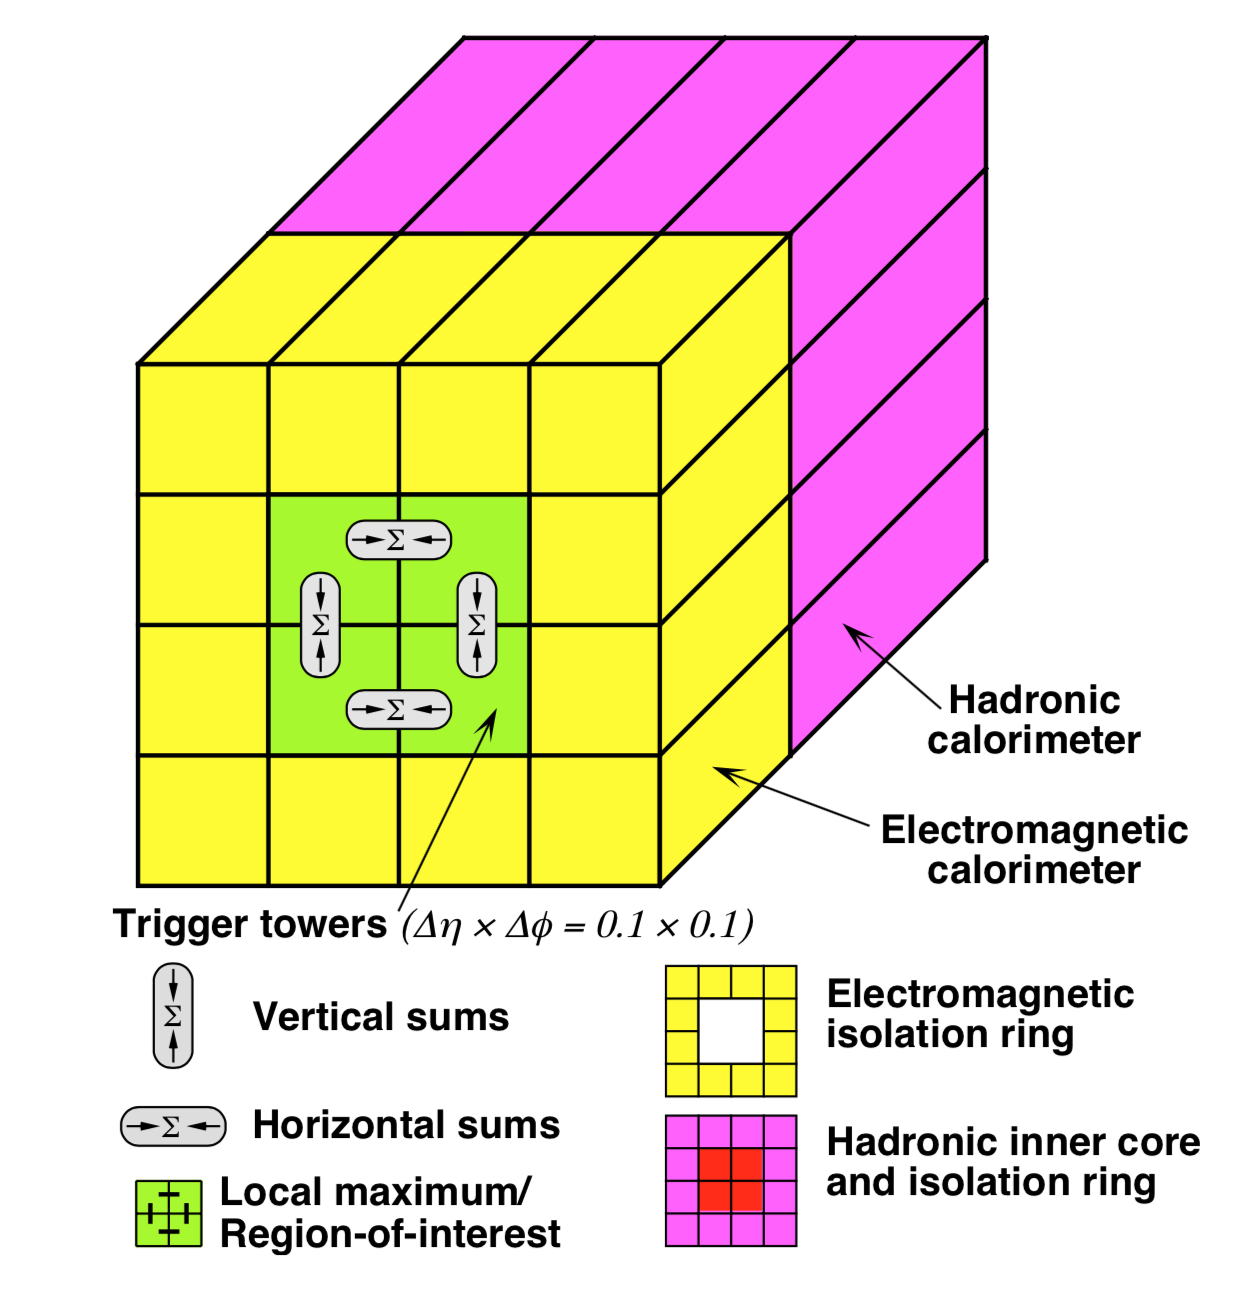
\includegraphics[width=.5\textwidth]{Trigger/cluster}
				\caption{\label{fig:calo_cluster} Illustration of the electron/photon and tau algorithms with the sums to be compared to programmable thresholds (from \cite{ATLASTrigger2010}).}
			\end{figure}


		\subsection*{The L1 Muon Trigger}

			The \ac{L1Muon} trigger system~\cite{ATLASPerf08} processes input data from fast muon trigger sub-detectors and its main task is to select muon candidates with a \pt\ threshold of 6 \GeV\ and identify the bunch crossing in which they were produced.

			Figure~\ref{fig:L1MuTrig} shows how muons are triggered at \ac{L1}. The \ac{RPC} system in the barrel region ($\abseta < 1.05$) and the \ac{TGC} system in the end-cap regions ($1.05 < \abseta < 2.4$) are employed. They provide a rough measurements of muon-candidate \pt, $\eta$, and $\phi$. Three planes in the barrel and three in each endcap form the trigger chambers. Each plane is comprised of two to four layers and muon candidates are identified by forming coincidences between the muon planes. Coincidences are formed requiring hits that lie within parametrised geometrical muon \emph{roads}. A road, as the example shown in Figure~\ref{fig:L1MuTrig}, essentially contains the trajectories, from the interaction point, of either positively or negatively charged muons with a \pt\ above a given threshold. In particular six programmable \pt\ thresholds are employed at \ac{L1}, divided into two sets: three low-\pt\ thresholds meant to cover values up to 10 \GeV, and three high-\pt\ thresholds meant to cover $\pt > 10 \GeV$.

			\begin{figure}[!htb]
				\centering
				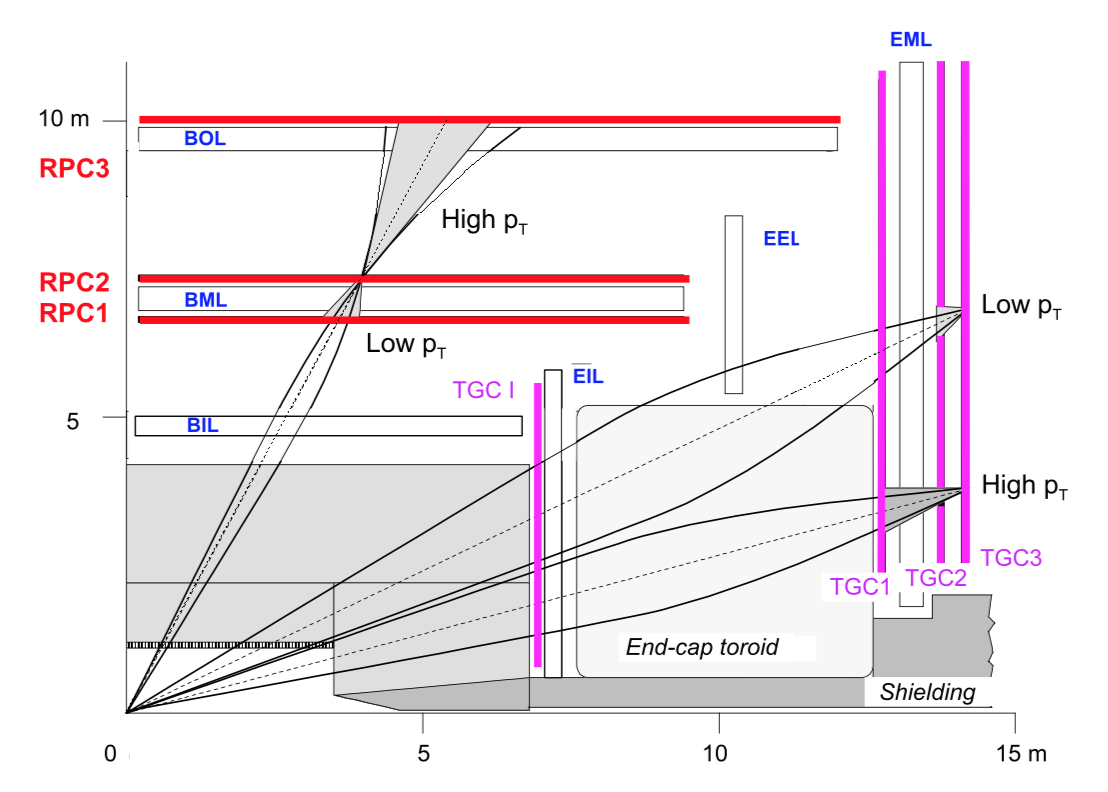
\includegraphics[width=\textwidth]{Trigger/L1MuTrigChambers}
				\caption{\label{fig:L1MuTrig} A schematic view of the \ac{L1Muon} trigger chambers (from \cite{ATLASTrigger2010}).}
			\end{figure}


		\subsection*{The CTP}

			The \ac{CTP}~\cite{ATLASJINST} applies the multiplicity requirements and pre-scale factors specified in the trigger menu to the inputs from the \ac{L1} trigger systems and forms the \ac{L1} trigger decision. Timing and control signals\footnote{The timing signals are defined with respect to the \ac{LHC} bunch crossings: a 25 ns time window centred on the instant at which a proton bunch might cross the \ac{ATLAS} interaction point.} are employed to distribute the \ac{L1} trigger decision to all \ac{ATLAS} sub-detector readout systems. It is responsible for applying the so-called \emph{preventive dead-time}, meant to limit the minimum time between two consecutive \ac{L1} accepts (\emph{simple dead-time}), $\mathcal{O}(100 \mathrm{ns})$, in order to both avoid overlapping readout windows, and restrict the number of \ac{L1} accepts allowed in a given number of bunch-crossings (\emph{complex dead-time}) to avoid buffers from overflowing. In addition, a \emph{busy dead-time}, can be introduced by \ac{ATLAS} sub-detectors to temporarily throttle the trigger rate. These dead-times are used to monitor the total \ac{L1} trigger rate, and individual trigger rates that need to be monitored before and after any pre-scales and/or any vetoes that have been applied. Furthermore, such information is also used to provide a measure of the \ac{L1} dead-time, which has to be accounted for when determining the luminosity~\cite{ATLASTrigger2010}.

		

			


	\section{High-Level Trigger}
	\label{sec:HLT}

		The events that are accepted by \ac{L1} are then buffered in the \ac{ROS} and processed by the \emph{High-Level Trigger} using information that is not available at \ac{L1}, such as finer-granularity calorimeter inputs, precision measurements from the \ac{MS} and tracking information from the \ac{ID}. \ac{HLT} receives \ac{RoI} from \ac{L1} and performs the reconstruction within them. As needed, the reconstruction performed by the \ac{HLT} software can either be run within \ac{RoI}s or performing a so-called \emph{full scan} of the detector. In order to reduce the processing time, a two-stage approach is employed for most \ac{HLT} triggers: a first reconstruction (fast) to reject the majority of events; a second precision reconstruction for the remaining events (slower). Events that are accepted by the \ac{HLT} get transferred to local storage at the experimental site and exported to the CERN’s computing centre for offline reconstruction~\cite{ATLASTrigger2015}. 

		
		\subsection{Inner detector tracking}
		\label{sec:tracking}

			The track reconstruction in the Inner Detector is a vital component of the trigger decision in the \ac{HLT}. A robust reconstruction of particle trajectories is an essential prerequisite for triggering on electrons, muons, taus, and $b$-jets. Furthermore, it is also used for triggering on inclusive \pp\ interactions and for the on-line determination of the beam spot\footnote{The luminous region produced by the collisions of proton beams.} where the reconstructed tracks provide the input for vertex reconstruction.

			The ID tracking in the trigger also includes information from the IBL, which significantly improves the tracking performance and in particular the impact parameter resolution~\cite{IBLTDR}. The tracking algorithms are called \emph{Fast Tracking} and \emph{Precision Tracking}. The former is comprised of trigger-specific pattern recognition algorithms, unlike the latter which is heavily based on offline-tracking algorithms.
			As already mentioned, once an \ac{RoI} has been identified by \ac{L1}, the algorithms are typically configured to run within it. Furthermore, in order to reduce CPU usage, the offline track-finding is seeded with tracks and space-points identified by fast tracking stage seeds. Running the full \ac{HLT} reconstruction for each event on an individual node, affords the opportunity to better optimise the \ac{RoI} geometry and use an advanced multi-stage strategy for the tau and $b$-jet triggers, which will be discussed in Section~\ref{sec:Trig_perf}. 

			In order to reduce the detector volume of \ac{RoI}, an advanced multi-stage approach, in particular for tau and \bj\ tracking, is employed. The first stage is to identify leading tracks within a long-in-$z$ but narrow-in-$\eta$ and $\phi$ \ac{RoI} running the \ac{FTF} algorithm. The leading tracks are used to construct a second-stage \ac{RoI}, constrained in both $\eta$ and $\phi$, but very tightly constrained in polar angle and with a small $z$ position width. The \ac{FTF} is then run again within the wider second-stage \ac{RoI}, followed by the Precision Tracking~\cite{ATLASTrigger2015,Miano:2016oty}. The second stage, the Precision Tracking, is heavily based on an optimised subset of the tracking algorithms used offline, which is slower than the first but, in return, it identifies objects constructed starting from the inner detector tracks.

			%As the future inclusion of the FTK tracks had to be taken into account, tracks provided by the FTK were integrated into the system although they were not used for any of the results presented in this work. 




		\subsection{Performance of HLT}
		\label{sec:Trig_perf}

			The performance of the tracking was estimated using 13-\TeV\ \pp\ collision collected in July 2015 by the \ac{ATLAS} detector, unless otherwise stated. In order to be as unbiased as possible, specific monitoring triggers that do not require a track to be present for the event to be accepted are used to estimate the efficiency of the tracking algorithms. All the quantities used to estimate the performance of the tracking, \ie\ efficiencies, residuals and resolutions, are calculated with respect to the tracks found by the offline reconstruction software. In particular, the efficiency is defined as the fraction of offline reference tracks that are matched to a trigger track 

			\begin{equation}
				\mathcal{E} = \frac{N_{\mathrm{trigger}}}{N_{\mathrm{offline}}}
				\label{eq:trig_eff}
			\end{equation}

			The tracking efficiency has been estimated for electrons and muons for the single-stage tracking, and for $b$-jets for the multi-stage approach, as part of the author's qualification task. The reconstructed tracks are required to have at least two (six) pixel (SCT) clusters and lie in the region $\abseta < 2.5$. The closest trigger track within a cone of size $\Delta R =  \Delta \eta^2 + \Delta \phi^2 = 0.05$ of the offline reconstructed track is selected as the matching trigger track.


			\subsubsection*{Electrons}

				Figure~\ref{fig:ele_idtrig_eff} shows the tracking efficiency for the 24 GeV electron trigger as a function of $\eta$ and \pt\ of the offline track. The tracking efficiency is measured with respect to offline tracks with $\pt > 20$ \GeV\ for tight offline electron candidates from the 24 GeV electron support trigger, which does not use the trigger tracks in the selection, despite being identical to the physics trigger. The \ac{FTF} and Precision Tracking efficiencies are all above 99\% within the whole pseudo-rapidity range. The small efficiency drop at low \pt\ is due to bremsstrahlung energy loss by electrons~\cite{ATLASTrigger2015}.

				\begin{figure}[!htb]
					\centering
					\subfloat[]{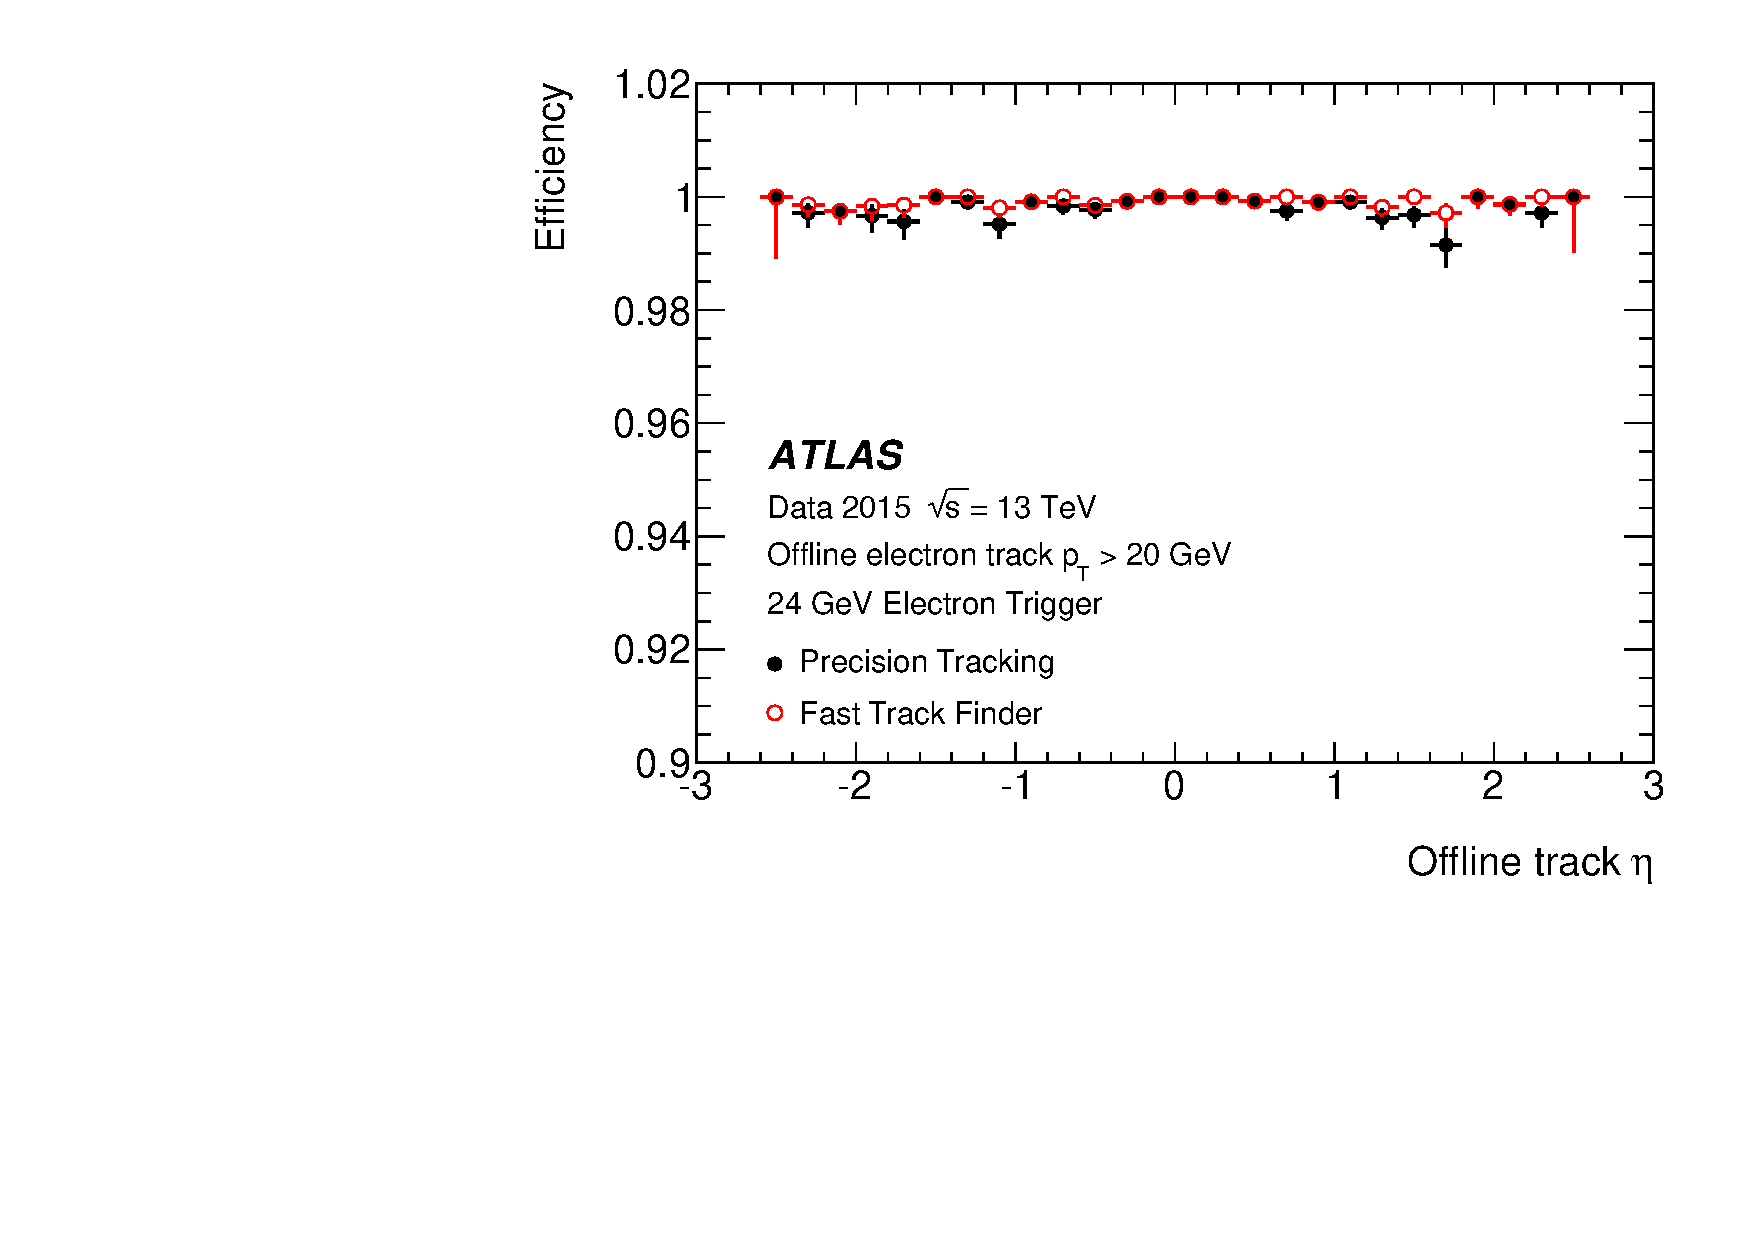
\includegraphics[width=0.5\textwidth]{Trigger/id/elec24plots3fb160224/HLT_eta_eff.pdf}}
					\subfloat[]{\includegraphics[width=0.5\textwidth]{Trigger/id/elec24plots3fb160224/HLT_pT_eff.pdf}}
					\caption{The ID tracking efficiency for the 24 \GeV\ electron trigger is shown as a function of the (a) $\eta$ and (b) $\pt$ of the track of the offline electron candidate. Uncertainties based on Bayesian statistics are shown (from~\cite{ATLASTrigger2015}).}
					\label{fig:ele_idtrig_eff}
				\end{figure}

			\subsubsection*{Muons}

				Figure~\ref{fig:idmuontriggera} shows the muon tracking performance with respect to offline muon candidates with $\pt > 6 \GeV$ selected by the 6 \GeV\ muon support trigger as a function of the offline muon \pt. The efficiency is well above 99\% in the entire \pt\ range for both \ac{FTF} and Precision Tracking. Figure~\ref{fig:idmuontriggerb} shows the resolution of the transverse track impact parameter with respect to offline as a function of the offline muon \pt. \ac{FTF} and Precision Tracking resolutions are better than 17 and 15 $\mu$m, respectively, for muon candidates with offline $\pt > 20 \GeV$. The difference ($\sim 10\%$) between the two algorithms is driven by the fact that Precision Tracking (black solid points) uses the space points found by the \ac{FTF} (red open points), but refits them using the offline algorithm. In other words, Precision Tracking runs a faster version of the full offline track fit and it performs better.

				\begin{figure}[!htb]
					\centering
					\subfloat[]{
					  \includegraphics[width=0.5\textwidth]{Trigger/id/mu6plots3fb/HLT_pT_eff.pdf}
					  \label{fig:idmuontriggera}
					}
					\subfloat[]{
					  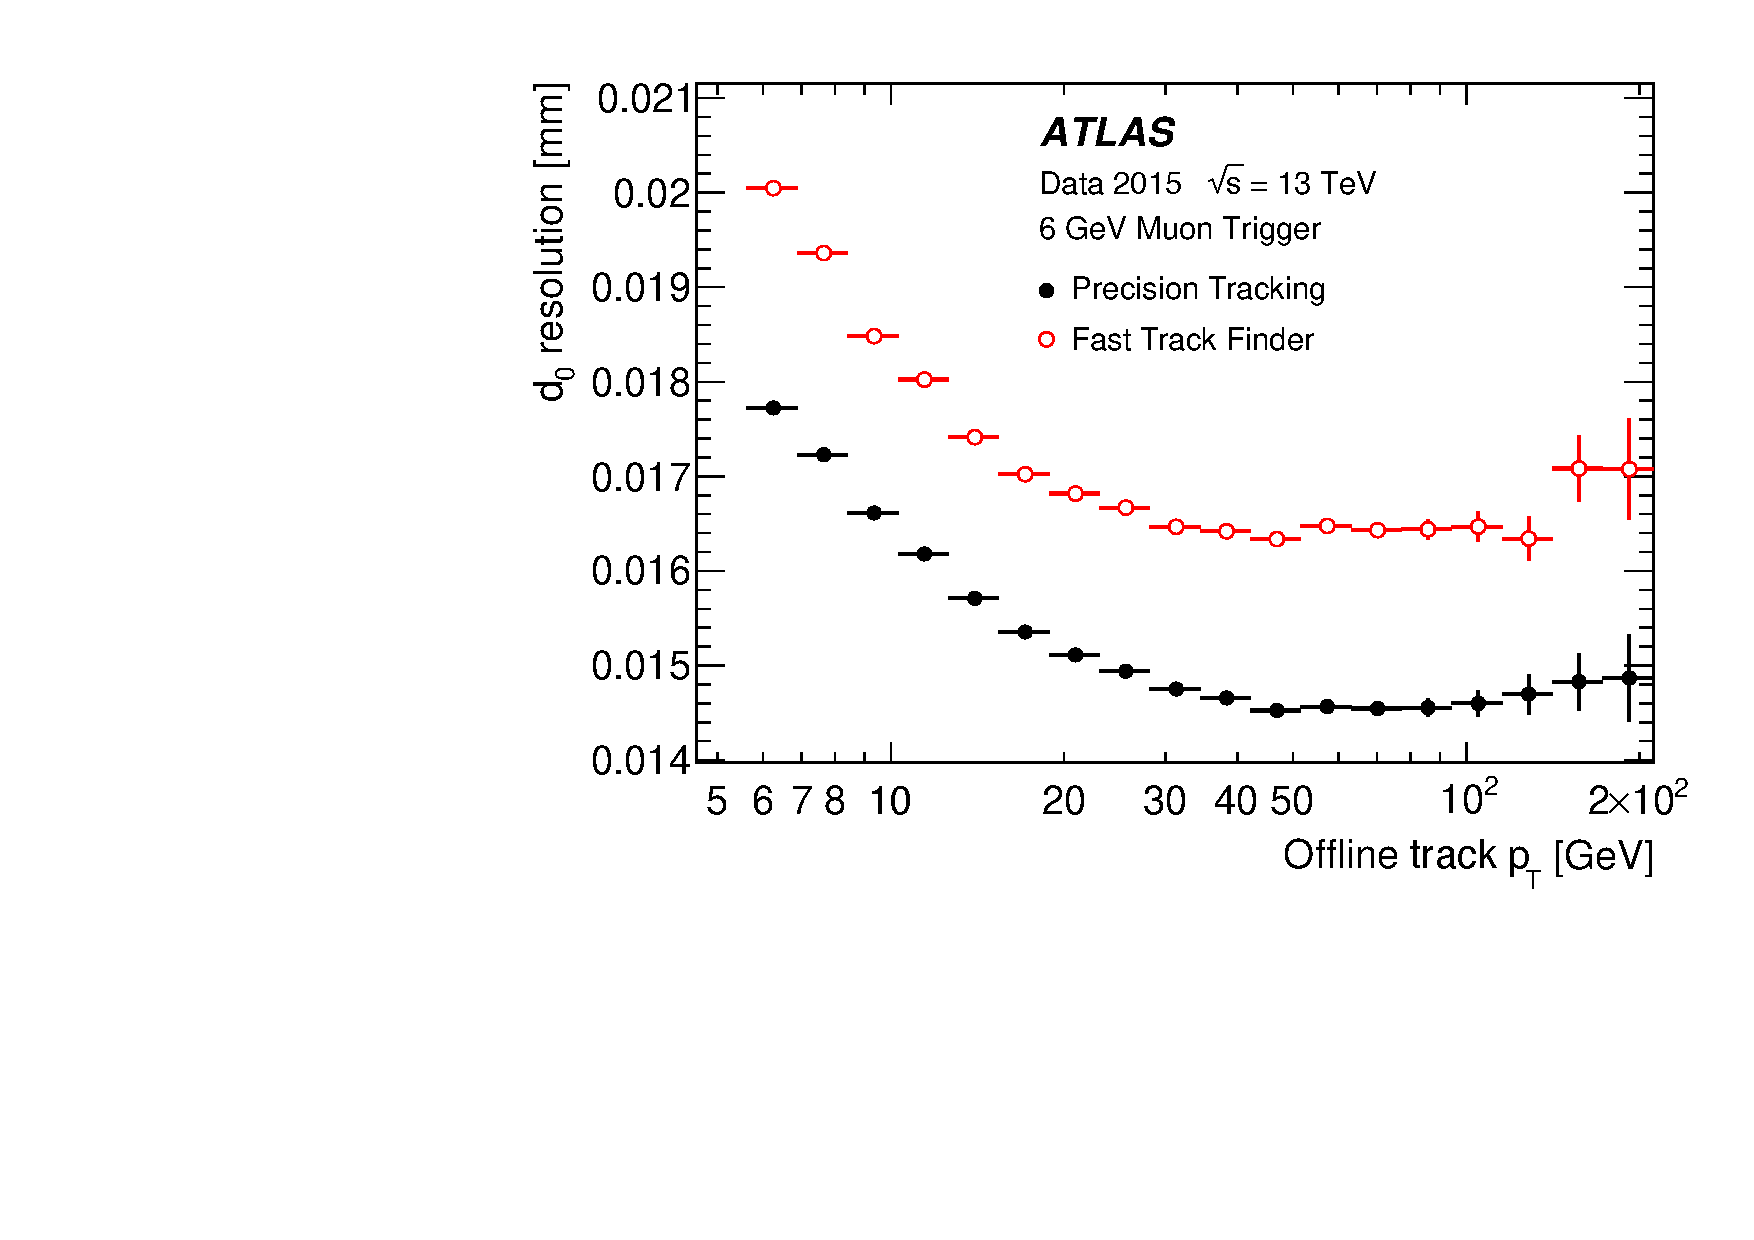
\includegraphics[width=0.5\textwidth]{Trigger/id/mu6plots3fb/HLT_rd0_vs_pt_sigma.pdf}
					  \label{fig:idmuontriggerb}
					}
					\caption{ 
					The ID tracking performance for the 6 \GeV\ muon trigger;
					(a) efficiency as a function of the offline reconstructed muon \pt,  
					(b) the resolution of the transverse impact parameter, $d_{0}$  as a function of the offline reconstructed muon \pt. Uncertainties based on Bayesian statistics are shown (from~\cite{ATLASTrigger2015}).}
				\label{fig:idmuontrigger}
				\end{figure}



			\subsubsection*{\emph{b}-jets}

				As previously mentioned, the $b$-jet triggers tracking algorithms are run in a larger \ac{RoI} than for electrons or muons and in order to limit CPU usage, multiple stage track reconstruction was implemented and deployed during Run-2.

				First, the leading track and its position along the beam-line are determined by executing fast tracking in an \ac{RoI} that is fully extended along the beam-line, in the $|z|<225$ mm region, but narrow (0.1) in both $\eta$ and $\phi$, as shown in the blue-shaded region in Figure~\ref{fig:idroi}. The second stage is then run, using this position along the beam-line, to reconstruct all tracks in an \ac{RoI} that is larger (0.4) in both $\eta$ and $\phi$ but limited to $|\Delta z|<10$ mm with respect to the leading track, as shown by the green-shaded region in Figure~\ref{fig:idroi}.

				\begin{figure}[!htb]
					\centering
					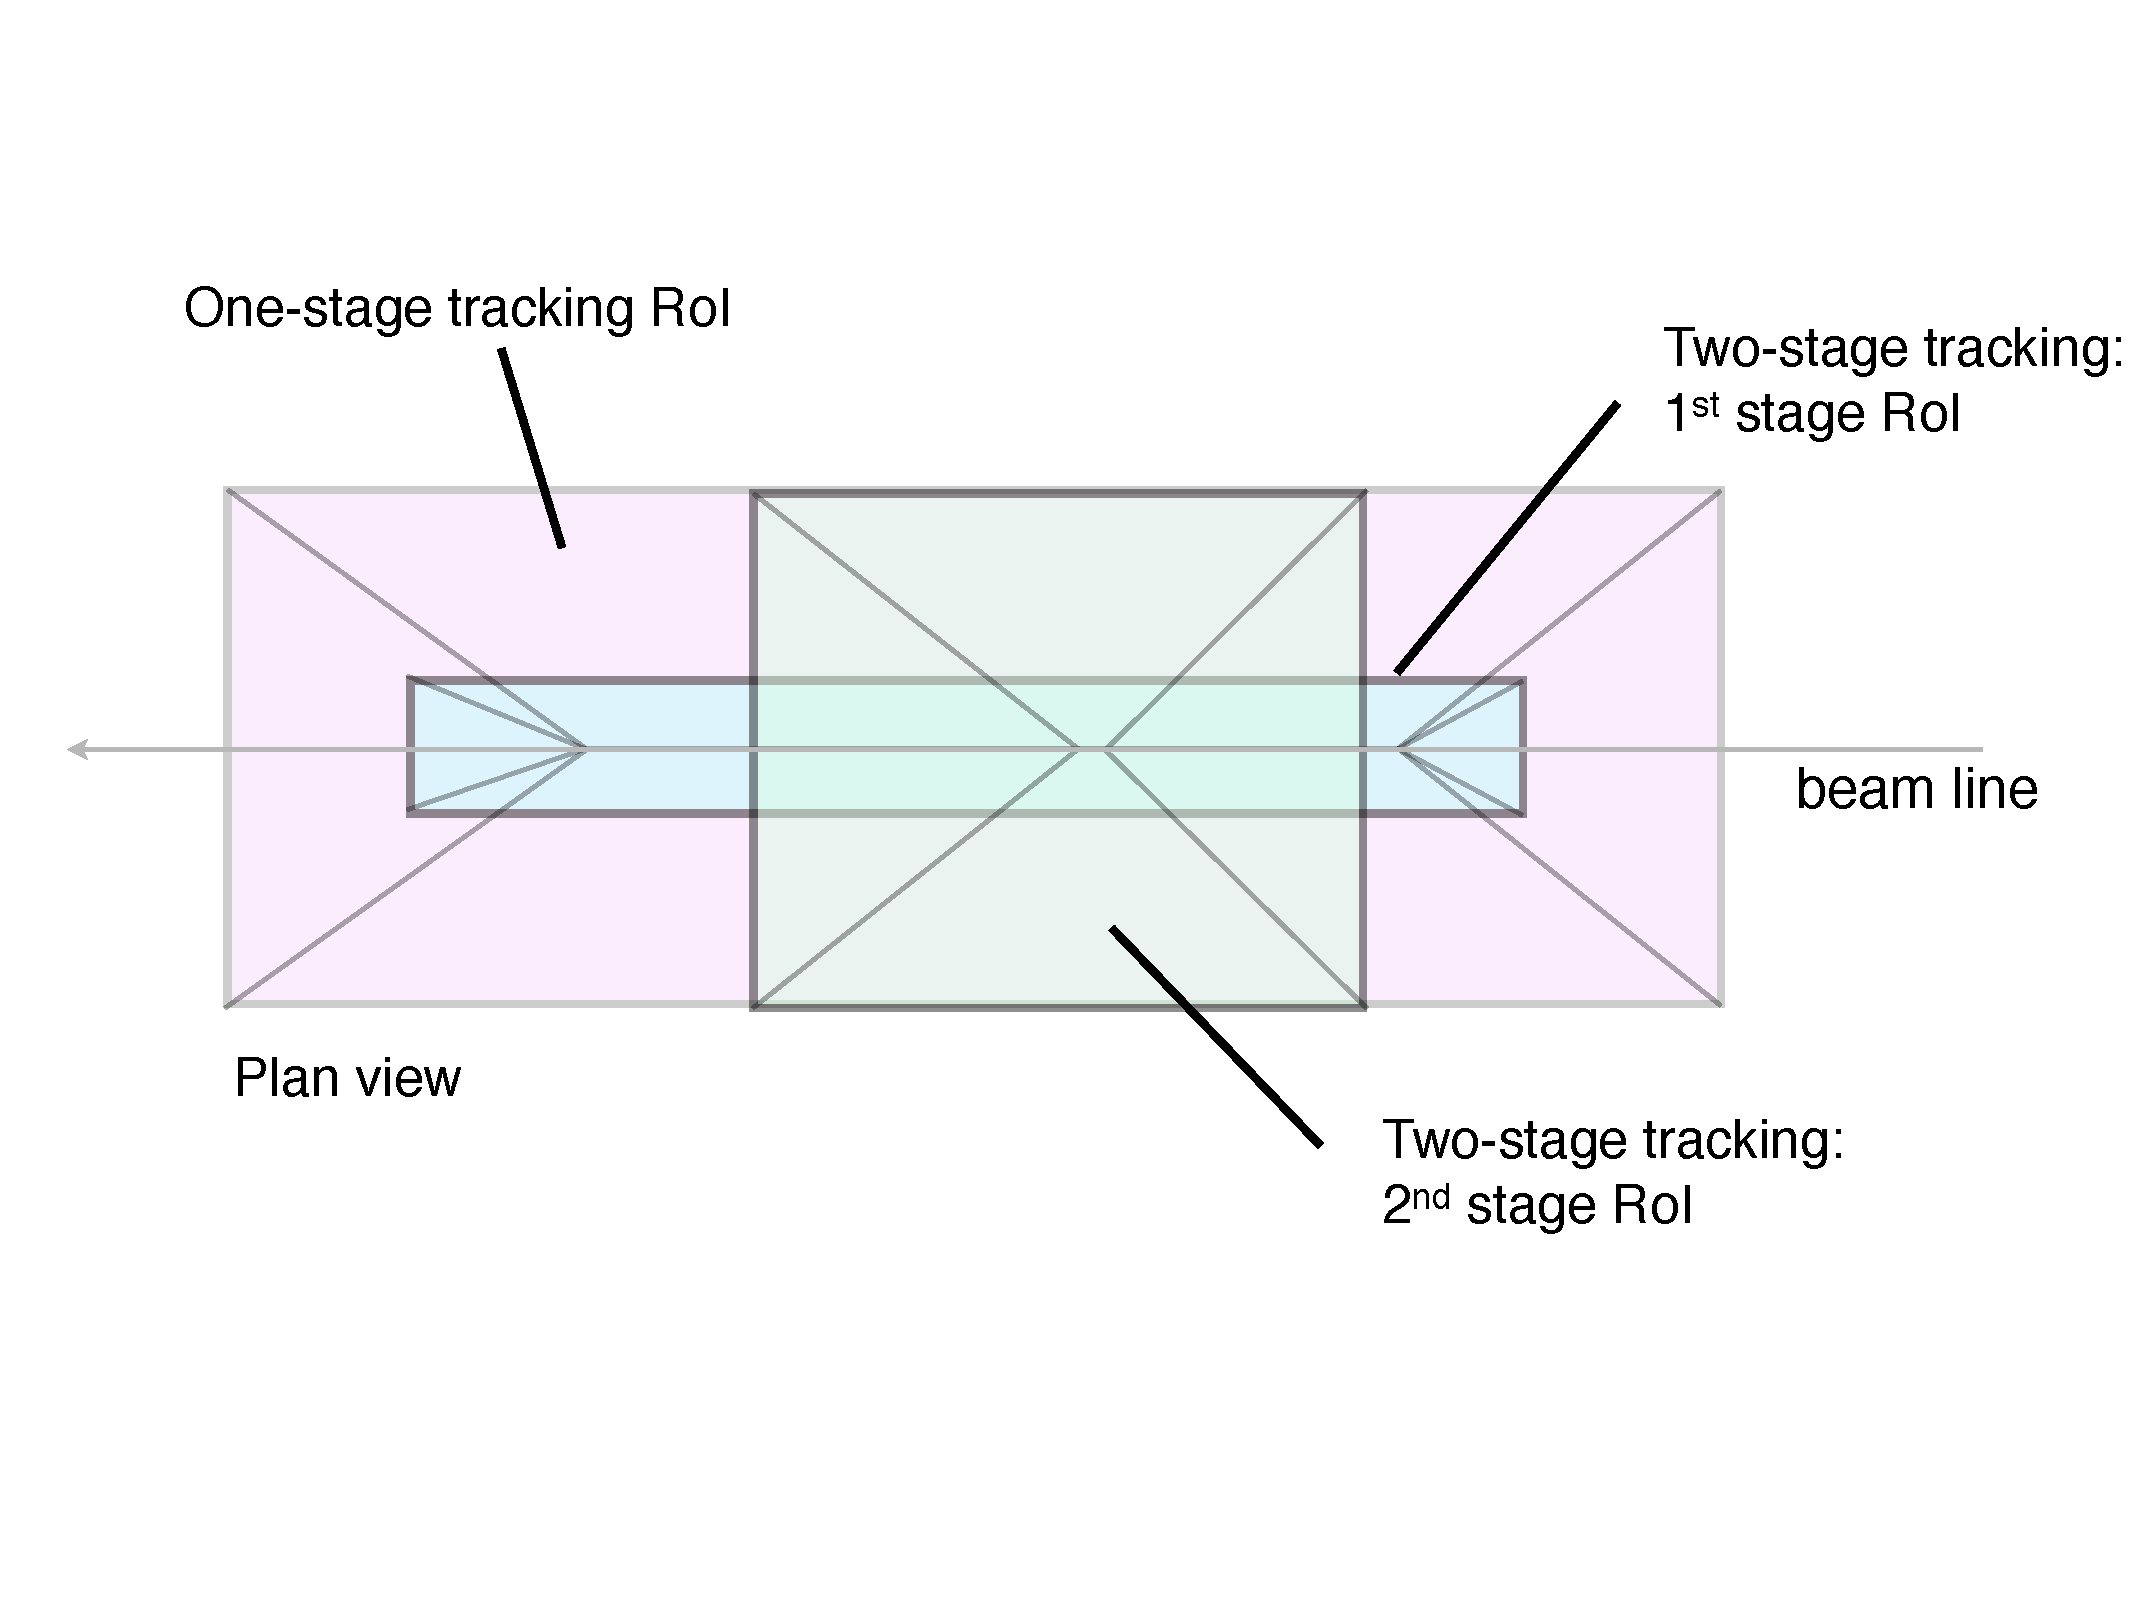
\includegraphics[width=0.65\textwidth]{Trigger/id/roi-plan}
					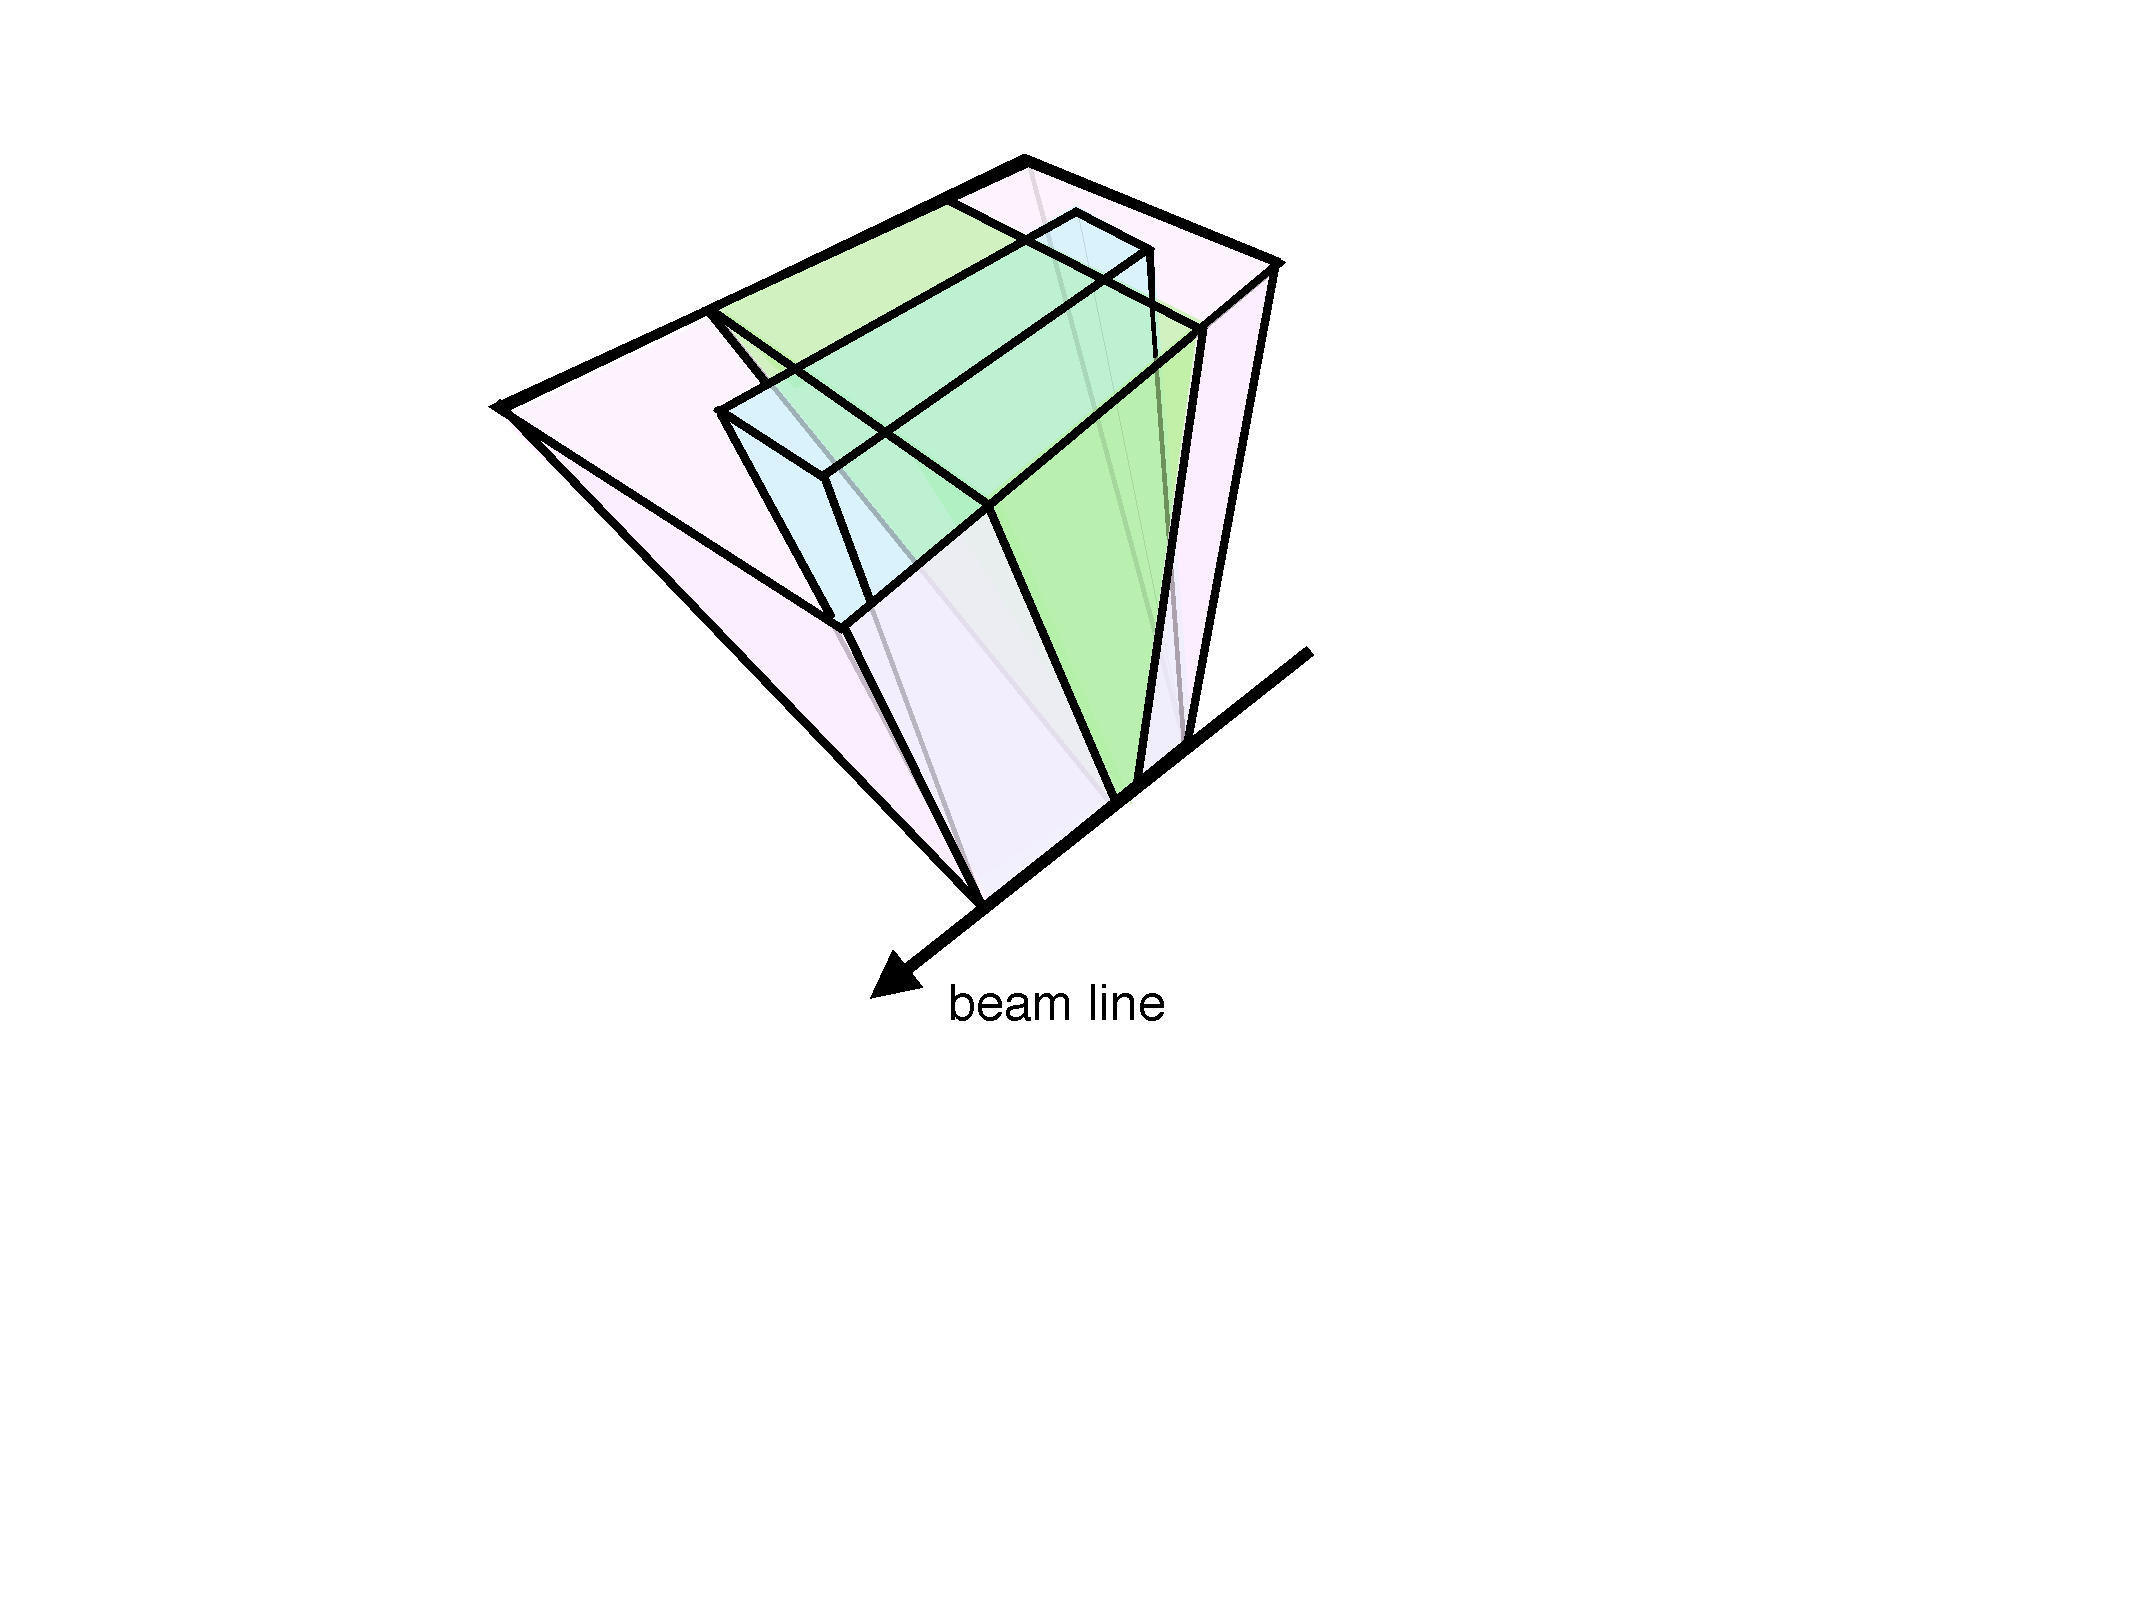
\includegraphics[width=0.3\textwidth]{Trigger/id/roi}
					\caption{An illustration of the \ac{RoI}s from the single-stage and two-stage tau lepton trigger tracking, shown in plan view (x-z plane) along the transverse direction and in perspective view. The z-axis is along the beam line. The combined tracking volume of the $1^{\mathrm{st}}$ and $2^{\mathrm{nd}}$ stage \ac{RoI} in the two-stage tracking approach is significantly smaller than the \ac{RoI} in the one-stage tracking scheme (from~\cite{ATLASTrigger2015}).}
					\label{fig:idroi}
				\end{figure}

				The first-stage vertex tracking takes all jets identified by the jet trigger with $\eta > 30$ \GeV\ and reconstructs tracks with the \ac{FTF} in a narrow region in $\eta$ and $\phi$ around the jet axis for each jet, but with $|z|<225$ mm along the beam line.
				
				Following this step, the primary vertex reconstruction~\cite{ATLAS-CONF-2010-069} is performed using the tracks from the fast tracking stage. This vertex is used to define wider \ac{RoI}s around
				the jet axes, with $|\Delta\eta|<0.4$ and $|\Delta\phi|<0.4$ but with $|\Delta z|<20$ mm relative to the primary vertex $z$ position. These \ac{RoI}s are then used for the second-stage 
				reconstruction that runs the fast track finder in the wider $\eta$ and $\phi$ regions followed by the Precision Tracking, secondary vertexing and $b$-tagging algorithms, which will not be discussed in this work.

				The performance of the primary vertexing in the $b$-jet vertex tracking can be seen in Figure~\ref{fig:bjetvertexa}, which shows the vertex finding efficiency with respect to 
				offline vertices in jet events with at least one jet with transverse energy above 55, 110, or 260 \GeV\ and with no additional $b$-tagging requirement. The efficiency is shown 
				as a function of the number of offline tracks with $\pt>1 \GeV$ that lie within the boundary of the wider \ac{RoI} (defined above) from the selected jets. The efficiency rises sharply and 
				is above 90\% for vertices with three or more tracks, and rises to more than 99.5\% for vertices with five or more tracks. The resolution in $z$ with respect to the offline $z$ position as shown in Figure~\ref{fig:bjetvertexb} is better than 100 $\mu$m for vertices with two or more offline tracks and improves to 60 $\mu$m for vertices with ten or more offline tracks.

				\begin{figure}[!htb]
					\centering
					\subfloat[]{
					  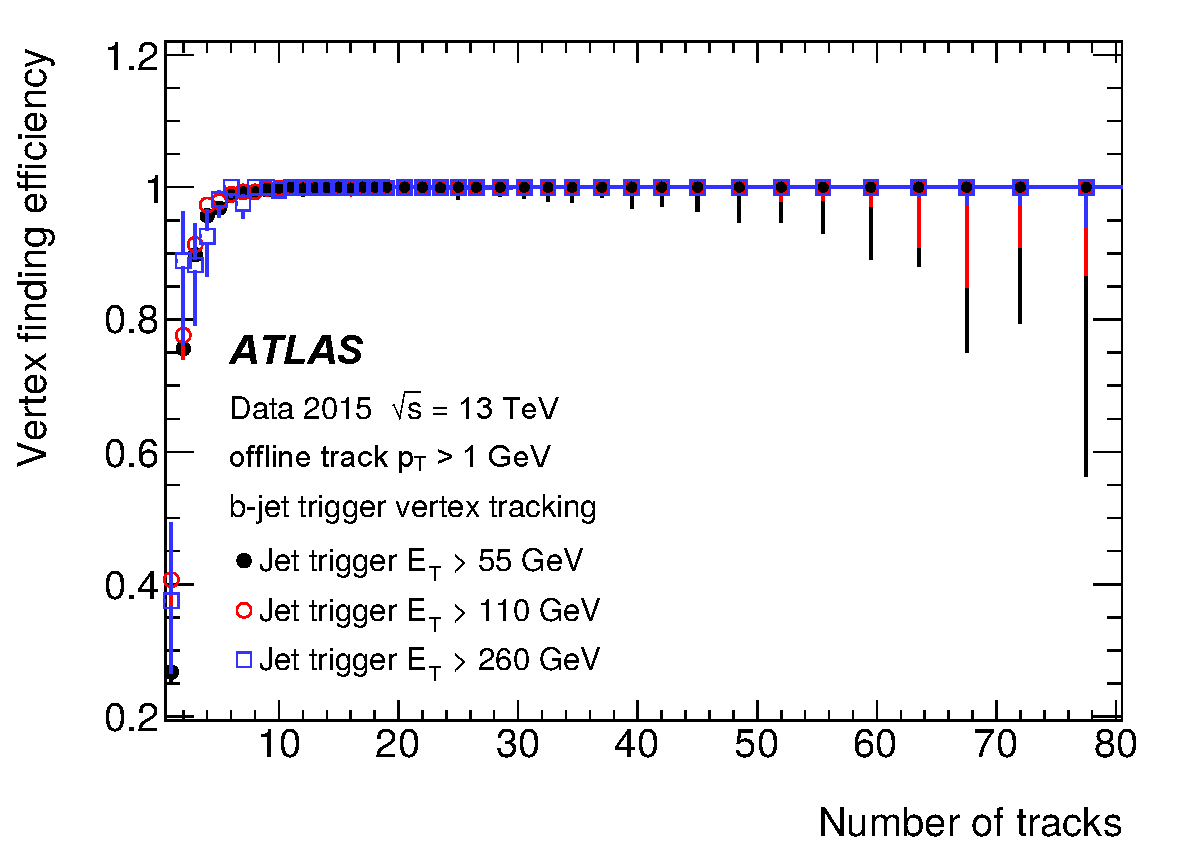
\includegraphics[width=0.5\textwidth]{Trigger/id/bjetvtx/HLT_xPrimVx_ntrax_eff.pdf}
					  \label{fig:bjetvertexa}
					}
					\subfloat[]{
					  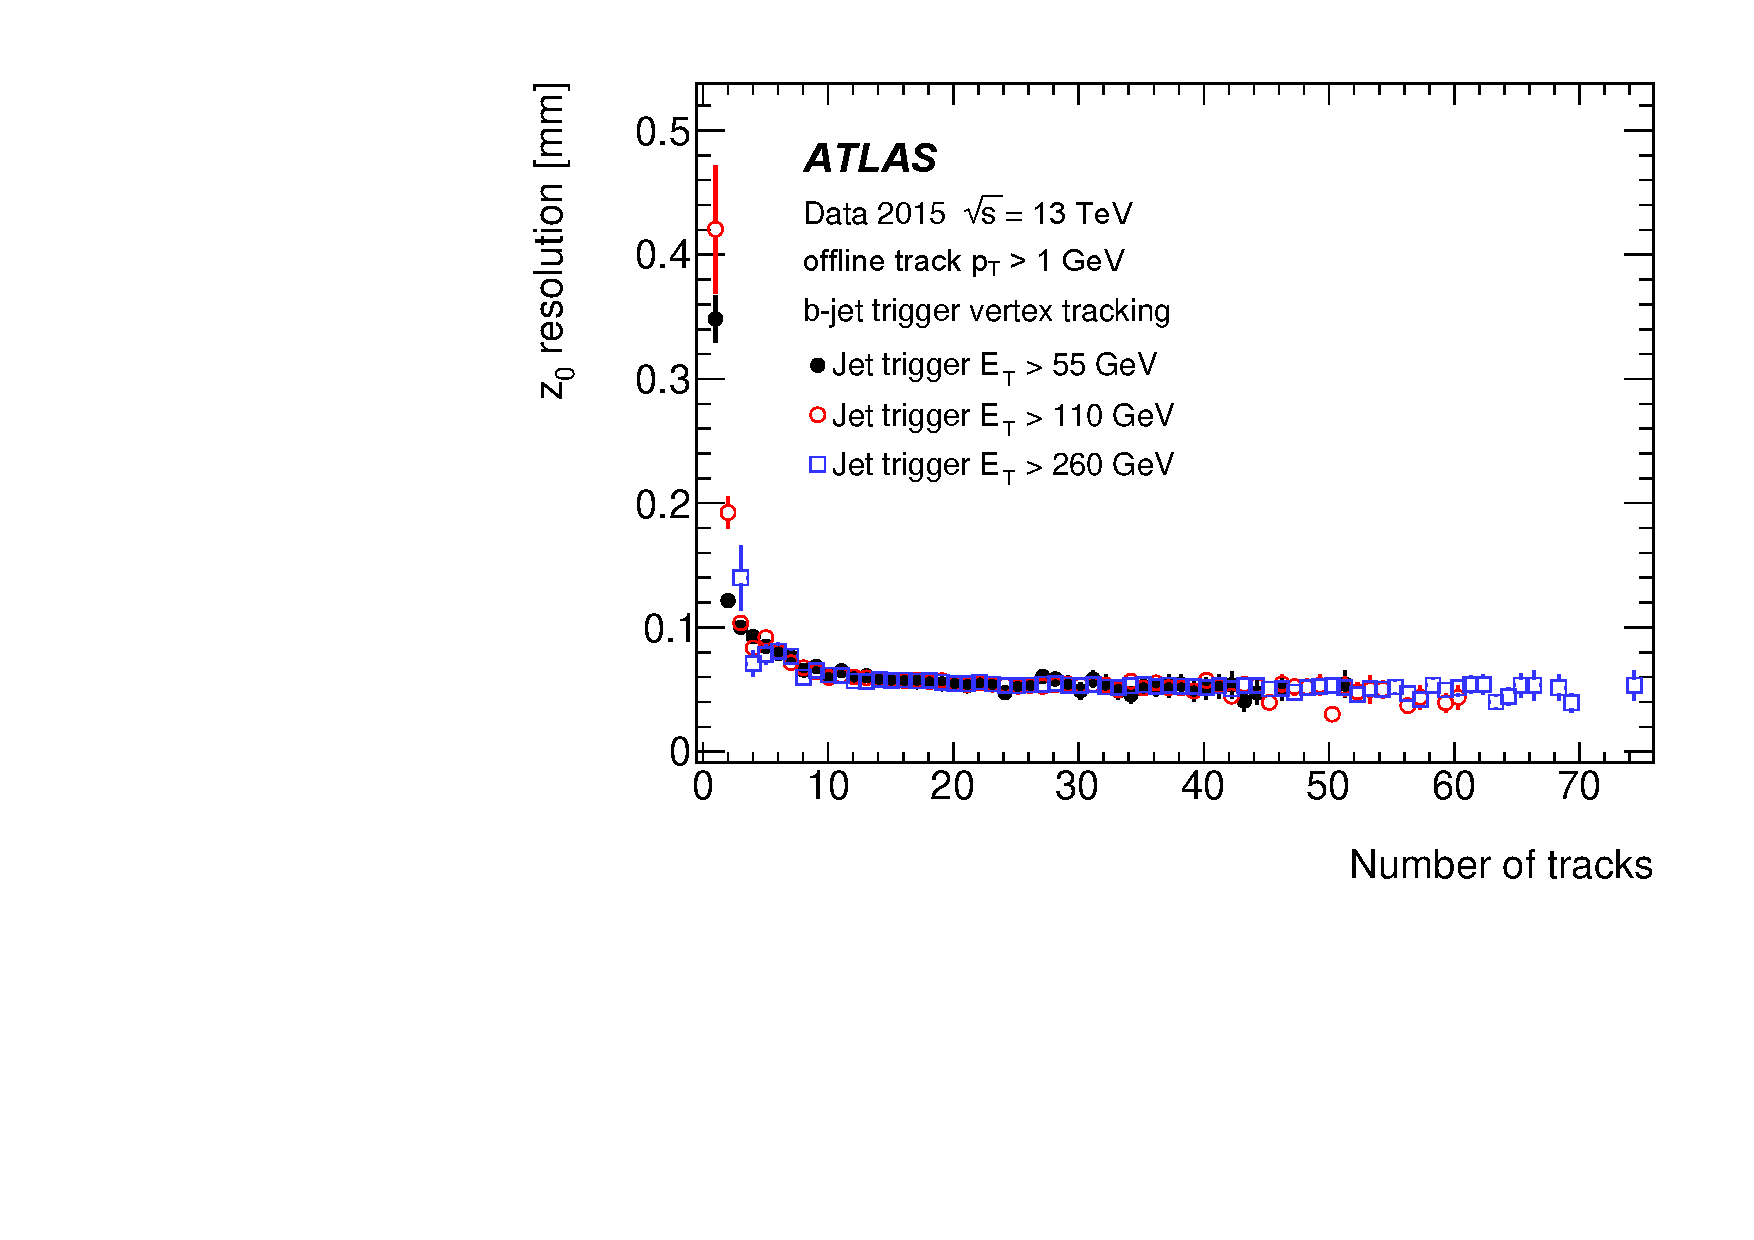
\includegraphics[width=0.5\textwidth]{Trigger/id/bjetvtx/HLT_xPrimVx_rdz_vs_ntrax_sigma.pdf}
					  \label{fig:bjetvertexb}
					}
					\caption{The trigger performance for primary vertices in the $b$-jet signatures for 55, 110 and 260 \GeV\ jet triggers; (a) the vertexing efficiency as a function of the number of offline tracks within the jets used for the vertex tracking, (b) the resolution in $z$ of the vertex with respect to the offline vertex position as a function of the number of offline tracks from the offline vertex (from~\cite{ATLASTrigger2015}).}
					\label{fig:bjetvertex}
				\end{figure}

			\subsubsection*{Missing Transverse Energy, \met}

				There exists several algorithms to reconstruct the \met\ at the \ac{HLT}. The \textit{missing} \HT\footnote{\HT\ is the scalar sum of the various \pt s in the event, $\displaystyle \HT = \sum_{i} \pt^i$.} (MHT) algorithm calculates \met\ as the negative sum of transverse energy of calibrated jets, constructed from calibrated topological clusters of calorimeter cells. This algorithm is the most relevant to the analysis presented in Chapter~\ref{ch:stop_ana}. The \textit{cell algorithm} is based on the negative sum of transverse energy deposited in calorimeter cells above a certain noise threshold. Unlike the cell algorithm, which calculates \met\ on the electromagnetic scale, the MHT algorithm looks at jets calibrated using jet energy scale, so that numerical threshold values for similar signal efficiencies differ. \textit{Pufit}, a third algorithm, was employed to disentangle calorimeter deposits from the hard-scatter, from those originating from pile-up interactions by grouping towers made out of topological clusters into a pile-up and a hard-scatter category. This grouping is based on their energy, where the threshold itself is dependent on the overall event activity measured by the total energy deposited in the calorimeter. The assumption is that the contribution to \met\ due to pile-up interactions is zero. Nevertheless a minimisation, which takes into account resolution terms, determines an effective energy density from pile-up interaction which allows a vanishing contribution to \met\ by the pile-up calorimeter towers. This correction is then subtracted from the hard-scatter towers. The negative sum of transverse energy of those pile-up corrected hard-scatter towers will provide the final \met\ value~\cite{ATL-COM-DAQ-2016-137}.

				Figure~\ref{fig:mettrigger} shows the turn-on curves for various \met\ triggers: Figure~\ref{fig:mettriggera} shows the efficiency as a function of \textit{modified}\footnote{To calculate the \met\ efficiency, \eg\ in events with muons, a muon trigger must be employed, therefore muon contributions are removed.} offline \met\ for three different \met\ trigger algorithms, using early 2016 \pp\ collision data. The events have been selected using single lepton (electron or muon) triggers. The x-axis shows the offline \met\ calculated from the sum of electrons, photons and jets, without the contributions from the muons. Three different \met\ high-level trigger algorithms are shown: \texttt{HLT\_xe80\_tc\_lcw\_L1XE50} calculates \met\ based on calibrated clusters of calorimeter cells, and has a threshold of 80 \GeV. \texttt{HLT\_xe90\_mht\_L1XE50} calculates \met\ based on reconstructed jets, and it has a threshold of 90 GeV. \texttt{HLT\_xe100\_L1XE50} calculates \met\ based on calorimeter cells calibrated at the electromagnetic scale, and has a threshold of 100 \GeV. All three algorithms are seeded by a Level-1 trigger algorithm with a threshold of 50 \GeV\ which is also shown; Figure~\ref{fig:mettriggerb} shows the combined \ac{L1} and \ac{HLT} efficiency of the missing transverse energy triggers \texttt{HLT\_xe110\_pufit\_L1XE50} and \texttt{HLT\_xe110\_mht\_L1XE50} as well as the efficiency of the corresponding \ac{L1} trigger (L1\_XE50) are shown as a function of the reconstructed \met\ (modified to count muons as invisible) using \pp\ collision data collected in 2017. The events shown are taken from data with a $\Wboson \to \ell \nu$ selection to provide a sample enriched in real \met. The \ac{HLT} \met\ of the \textit{pufit} algorithm is calculated as the negative of the transverse momentum vector sum of all calorimeter topological clusters corrected for pileup. The pileup correction is done by grouping the clusters into coarser “towers” which are then marked as pileup if their $E_\mathrm{T}$ falls below a pileup-dependent threshold.

				\begin{figure}[!htb]
					\centering
					\subfloat[]{
					  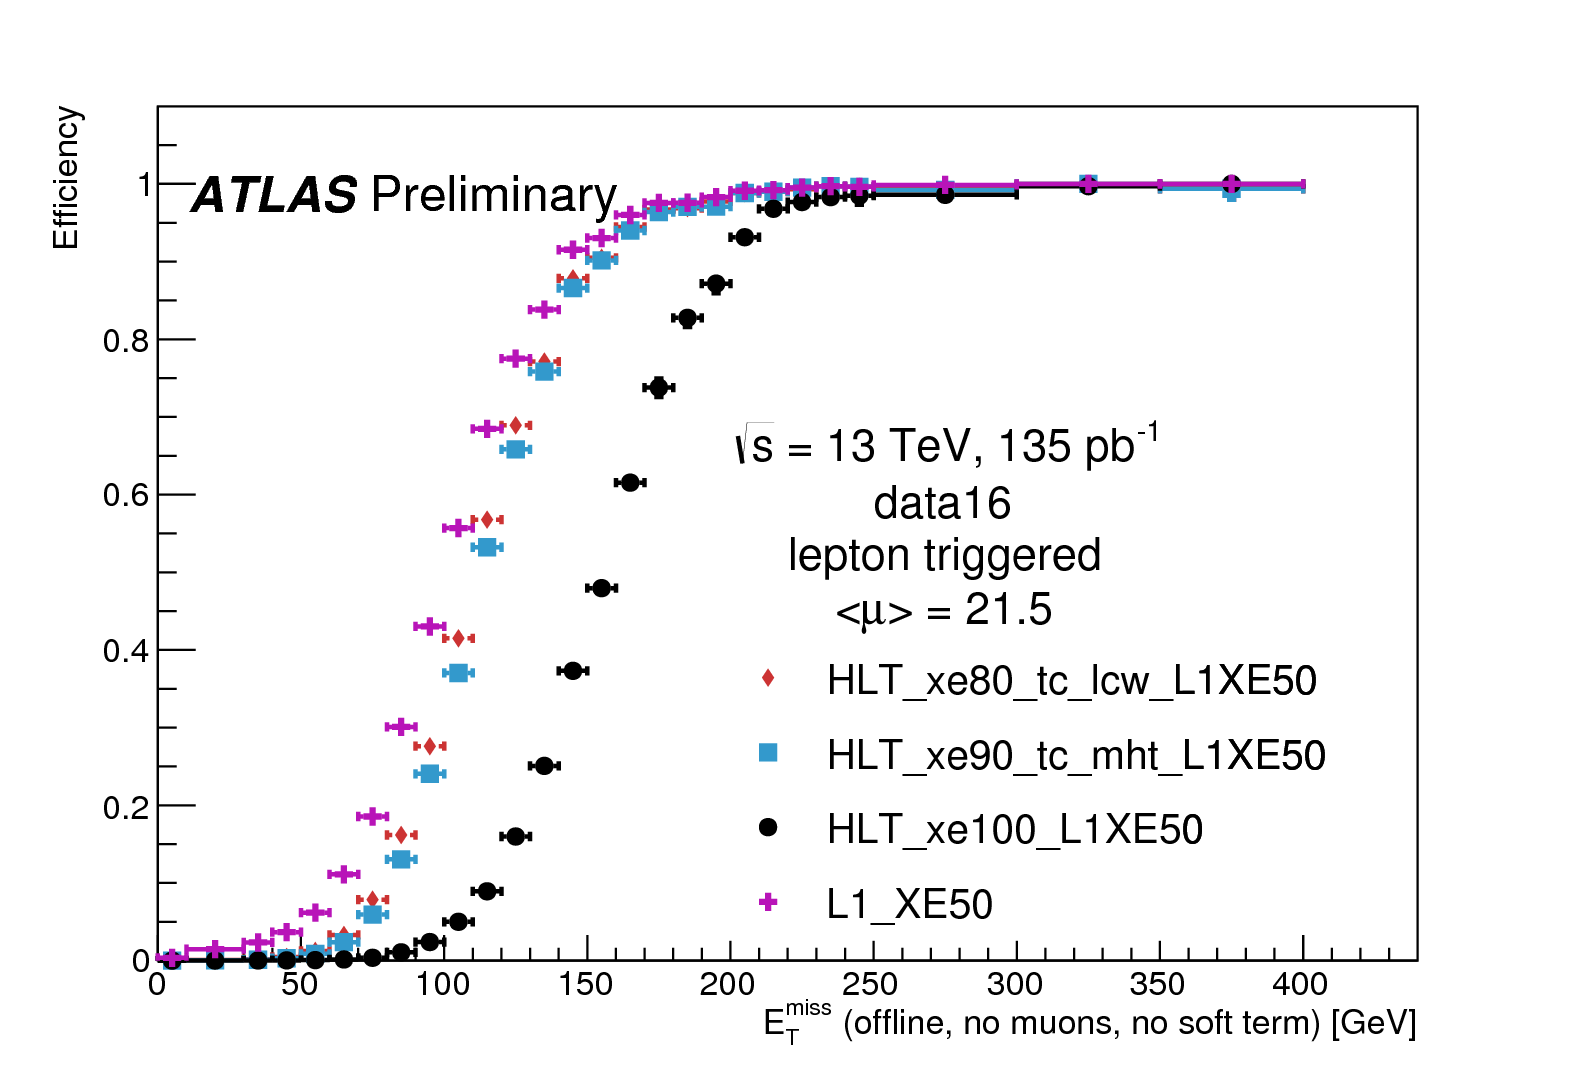
\includegraphics[width=0.5\textwidth]{Trigger/hlt_met_unprescaled2016.png}
					  \label{fig:mettriggera}
					}
					\subfloat[]{
					  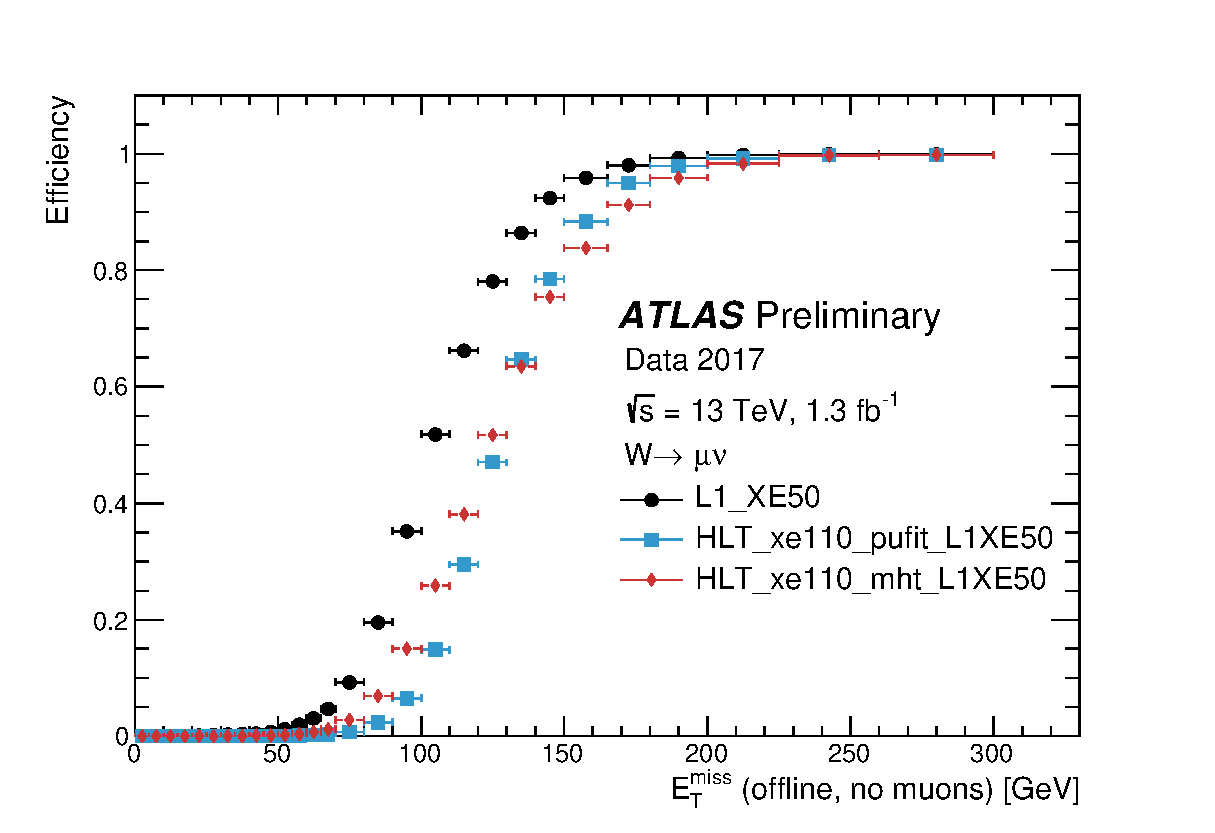
\includegraphics[width=0.5\textwidth]{Trigger/hlt_met_unprescaled2017.eps}
					  \label{fig:mettriggerb}
					}
					\caption{Turn-on curves of various \met\ triggers: Figure~\ref{fig:mettriggera} shows the efficiency as a function of offline \met\ for three different \met\ trigger algorithms. Three different \met\ high-level trigger algorithms are shown: \texttt{HLT\_xe80\_tc\_lcw\_L1XE50} calculates \met\ based on calibrated clusters of calorimeter cells, and has a nominal threshold of 80 \GeV. \texttt{HLT\_xe90\_mht\_L1XE50} calculates \met\ based on reconstructed jets, and has a nominal threshold of 90 \GeV. \texttt{HLT\_xe100\_L1XE50} calculates \met\ based on calorimeter cells calibrated at the electromagnetic scale, and has a nominal threshold (at the electromagnetic scale) of 100 \GeV. All three algorithms are seeded by a Level-1 trigger algorithm with a nominal threshold of 50 \GeV\ which is also shown; Figure~\ref{fig:mettriggerb} shows missing transverse energy trigger efficiencies for \texttt{HLT\_xe110\_pufit\_L1XE50} and \texttt{HLT\_xe110\_mht\_L1XE50} and for the corresponding \ac{L1} seed (\texttt{L1\_XE50}). (from~\cite{ATLASMETTriggerPublicPage}).}
					\label{fig:mettrigger}
				\end{figure}
